\documentclass[a4paper]{article}

\usepackage[english]{babel}
\usepackage[utf8x]{inputenc}
\usepackage{amsmath}
\usepackage{amsfonts}
\usepackage{graphicx}
\usepackage[]{algorithm2e}
\usepackage[colorinlistoftodos]{todonotes}

\title{CS 5785 -- Applied Machine Learning -- Lec.\ 17}
\author{Prof.\ Nathan Kallus, Cornell Tech\\Scribe: TBD}
\date{Oct.\ 31, 2017 (Under construction)}

\begin{document}
\maketitle

\section{CART Recap}
Recall the following pros and cons of Classification and Regression Trees.
\\
\\
Pros:
\begin{itemize}
\item Easy to interpret
\item Readily handles mixed discrete and continuous inputs (example: in a survey)
\item Insensitive to monotone transformations on input (since we are sweeping from minimum to maximum of the range.)
\item Performs automatic variable selection
\item Some robustness to outliers
\item Can be modified to handle missing inputs
\end{itemize}
Cons:
\begin{itemize}
\item Accuracy is not as high as competing methods
\item Instability in hierarchy: a bad split propagates the error down to all the splits below it
\end{itemize}

The worst of the cons is \textit{instability}. Instability can be addressed through a technique called \textit{bagging}, or bootstrap aggregating, which will lead us to the concept of \textit{Random Decision Forests}.

\section{Random Decision Forests}
Both in machine learning and in biology forests are defined in the same way:
\newenvironment{definition}[1][Definition]{\begin{trivlist}
\item[\hskip \labelsep {\bfseries #1}]}{\end{trivlist}}

\begin{definition}
A \underline{forest} is a set of trees.
\end{definition}

Random Decision Forests (also called Random Forests) were first proposed as a technique for handwritten digit classification (see Fig.~\ref{fig:randomforest}).  More recently they were used for human body pose estimation in Microsoft Kinect.  The key idea is to use not one but many trees, each grown on different subsets of the data, to conquer the instability problem mentioned above.

\begin{figure}
\centering
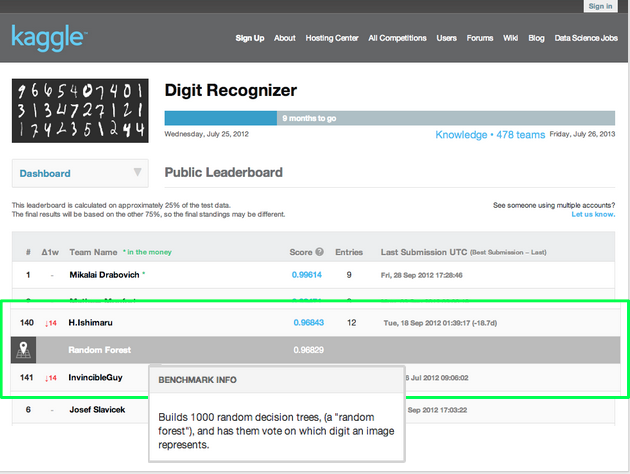
\includegraphics[width=0.75\textwidth]{RandomForests.png}
\caption{\label{fig:randomforest}Random Forest classification, shown here as a baseline approach for a digit recognition challenge, is a popular method on Kaggle.}
\end{figure}


The process of creating a random forest is as follows.
\begin{itemize}
\item Train $B$ different trees on different subsets of the data, sampling with replacement (allowing reuse of some data)
\item Produce an ensemble of trees $\{T_b\}_1^B$
\item To make a prediction at a new point $x$, 
\begin{itemize}
\item For regression use: $${\hat f}_{rf}^B=\frac{1}{B}\sum_{b=1}^B T_b(x)$$
\item For classification, let ${\hat C}_{b}(x)$ be the class prediction of the $b$th random forest tree. Then:
$${\hat C}_{rf}^B=\text{majority vote}\{{\hat C}_b(x)\}_1^B$$
\end{itemize}
\end{itemize}

Up to this point this is just ``bagging,'' or boostrap aggregation, simply rerunning the same learning algorithm on different subsets of the data.  This can result in highly correlated predictors, limiting the amount of variance reduction. We need to decorrelate the base learners.  We do this as follows. Before each split, select $m\leq p$ of the input variables at random as candidates for splitting.  A typical value for $m$ is $\sqrt p$. By choosing to get a sub-set of feature variables, we coerce the decision trees to become as diverse as possible. This helps us to obtain trees that have learnt some features better than the others, and avoid growing similar trees everytime.

\begin{figure}
\centering
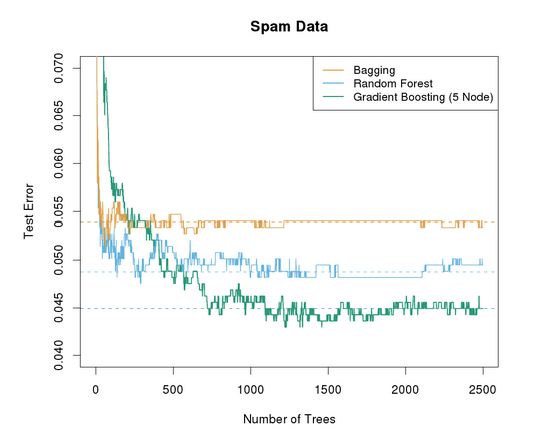
\includegraphics[width=0.85\textwidth]{Fig151.png}
\caption{\label{fig:fig151}HTF Figure 15.1 }
\end{figure}

Fig.~\ref{fig:fig151} shows us the performance benefit of using Random Forests compared to Bagging.

\section{Boosting}
Boosting, one of the most influencial machine learning ideas of the last 20 years, was originally designed for classification but can be extended to regression. The basic idea behind boosting is to combine the outputs of many \textit{weak} classifiers to produce a powerful \textit{commitee}. Boosting is superficially related to bagging, since they both combine outputs from many classifiers, but is in fact fundamentally different. 

\begin{definition}
A \underline{weak classifier} is a classifier with an error rate only slightly  better than guessing.
\end{definition}

The most popular implementation of a boosting algorithm is AdaBoost.M1 (Freund and Schapire 1997), see Fig.~\ref{fig:adaboost}. 

\begin{figure}
\centering
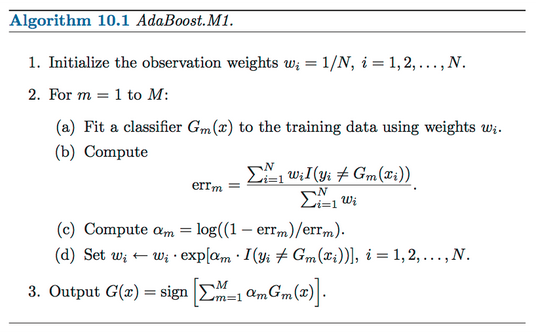
\includegraphics[width=0.85\textwidth]{adaboost.png}
\caption{\label{fig:adaboost}The ADABoost.M1 Algorithm }
\end{figure}

Consider the 2-class case with output variable coded $Y\in \{-1,1\}$. Classifier $G(X)$ produces a prediction taking value $1$ or $-1$. The error rate on the training data is defined as:
$$\overline{err}=\frac{1}{N}\sum_{i=1}^N I(y_i\neq G(x_i))$$
The expected error rate on future predictions (i.e., on the testing data) is defined as:
$$E_{XY}I(Y\neq G(X))$$

The idea behind boosting is to apply many weak classifiers  sequentially to successively modified versions of the data, producing a sequence of weak classifiers $G_m(x)$, $m=1,2,\ldots,M$.  We combine all of these predictions using a weighted majority vote:
$$G(x)=\text{sign}\left(\sum_{m=1}^M \alpha_m G_m(x)\right)$$
%Where the $\alpha_m$s are the weights of the weak classifiers computed by the algorithm and $w_i$s are the weights of the observations.
The weights $\alpha_1,\alpha_2,\ldots,\alpha_M$ are computed by the boosting algorithm (AdaBoost.M1).
\newline
%The algorithm gives a higher weight to the more accurate classifiers, such that if $\overline{err}(G_i(X))\geq\overline{err}(G_j(X))$ then $\alpha_i\geq\alpha_j$.

\begin{figure}
\centering
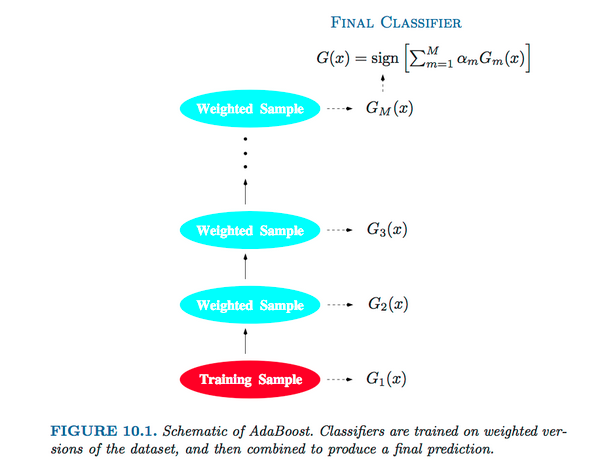
\includegraphics[width=0.75\textwidth]{Boosting.png}
\caption{\label{fig:boosting}}
\end{figure}

In Fig.~\ref{fig:boosting} we see the pipeline of the boosting meta-algorithm.\footnote{We call it a meta-algorithm since it operates on top of our choice of $G(\cdot)$, which is itself an algorithm.} The training sample gets successively reweighted, producing one weak classifier at a time. The pipeline is:
\begin{enumerate}
\item Initially we set the weights on the training observations $(x_i,y_i)$ all to $w_i=\frac{1}{N}$, meaning the first step trains the classifier in the usual fashion with equal weights on all data points.
\item On iterations $m=2,3,\ldots,M$, the observations' weights are individually modified and the classification algorithm is reapplied. The modification is done such that at step $m$, the observations that were misclassified by $G_{m-1}$ get increased weights and the opposite for observations correctly classified. In this sense, we focus our effort on observations that failed previously.
\item As iterations proceed, difficult observations recieve ever-increasing influence such that each successive classification is forced to concentrate on training observations missed by previous ones in the sequence.
\end{enumerate}

In Fig.~\ref{fig:boosting}, step 2a we fit a new classifier based on the current weights. In step 2b we compute the normalized  error rate of the classifier. In step 2c we calculate $\alpha_m$ and in step 2d we recalculate the weights. Finally, the algorithm outputs the sign of the sum of all classifier results. 

\subsection{Synthetic Example}
To build intuition, consider the following synthetic example from HTF Sec.~10.1.  Prepare a set of randomly sampled feature vectors $X\in\mathbb{R}^p$ with $X\sim\mathcal{N}(0,I)$ and $p=10$.  Define a deterministic target $Y$ as follows:
\begin{displaymath}
   Y = \left\{
     \begin{array}{lr}
       1 & \text{if}\quad \sum_{j=1}^{10} X_j ^2> \chi_{10}^2(0.5)\\
       0 & \text{otherwise}
     \end{array}
   \right.
\end{displaymath} 
Recall that the $\chi^2$ random variable arises from the sum of standard normal random variables, the number of random variables in this sum is equal to the degrees of freedom.  The value $\chi_{10}^2(0.5)=9.34$ is the median of a $\chi^2$ random variable with $10$ degrees of freedom.  For purposes of visualization, in the case of $p=2$ the decision boundary would be a circle with the $Y=1$ observations outside the circle and the $Y=0$ observations inside.

Assume there are $2000$ training observations ($N=2000$), with approximately $1000$ observations in each class (evenly distributed), and $10,000$ test observations. For the weak classifier we will use something called a \textit{stump}.

\begin{definition}
A \underline{stump} is a special case of a decision tree that uses only one input dimension and only one split node (see Fig.~\ref{fig:stump}).
\end{definition}

\begin{figure}
\centering
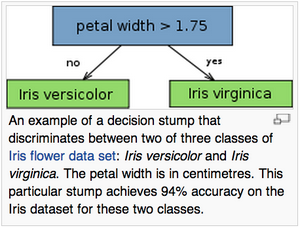
\includegraphics[width=0.75\textwidth]{stump.png}
\caption{\label{fig:stump}[Wikipedia]}
\end{figure}

Recall that after we create the training data in this synthetic example, we pretend we know nothing about how it was made, we're just handed $2000$ training observations in the form $(x_i,y_i)$ with a $50/50$ class split and we want to train a classifier on it. The stump we will use as a weak classifier has the form
\begin{displaymath}
   G(x|j,\theta) = \left\{
     \begin{array}{lr}
       1 & \text{if}\quad x_j \leq \theta\\
       -1 & \text{otherwise}
     \end{array}
   \right.
\end{displaymath} 
The parameters are $j$ and $\theta$.  (We are free to flip the sign or use $x_j \geq \theta$.)  Training the stump just amounts to stepping through $j=1,\ldots,p$ and empirically choosing the best threshold $\theta$ based on the training error. Unsurprisingly, if we fit one stump to the training data we'll get an error rate close to chance (50\%).  In the next lecture we'll see how much the performance improves as we add more stumps using AdaBoost.

\end{document}
